\documentclass{article}
\usepackage[final]{neurips_2024}

\usepackage[utf8]{inputenc}
\usepackage[T1]{fontenc}
\usepackage{hyperref}
\usepackage{url}
\usepackage{booktabs}
\usepackage{amsfonts}
\usepackage{amsmath}
\usepackage{nicefrac}
\usepackage{microtype}
\usepackage{xcolor}
\usepackage{graphicx}
\usepackage{subcaption}

\graphicspath{{../figures/}}

\title{Pixel-Space Posterior Sampling for Image Deblurring:\\
       A Controlled Comparison of DPS and FlowDPS-Style Guidance\\
       on CelebA-HQ-256}

\author{%
  Eeman Adnan \\
  Department of Artificial Intelligence \\
  Lahore University of Management Sciences \\
  \texttt{24280022@lums.edu.pk} \\
  \And
  Muhammad Aslam Adnan \\
  Department of Artificial Intelligence \\
  Lahore University of Management Sciences \\
  \texttt{25280067@lums.edu.pk} \\
  \And
  Mufaddal Hatim \\
  Department of Artificial Intelligence \\
  Lahore University of Management Sciences \\
  \texttt{25280084@lums.edu.pk} \\
}

\begin{document}
\maketitle

\begin{abstract}
We present a controlled, pixel-space comparison of two posterior
sampling paradigms for image deblurring on CelebA-HQ-256 faces:
\emph{Diffusion Posterior Sampling} (DPS) on a CelebA-HQ-256 DDPM
and a from-scratch pixel-space reimplementation of \emph{FlowDPS}
on the Liu et~al.\ 2023 Rectified Flow checkpoint. Across an
18-condition matched-Gaussian grid (1,800 reconstructions),
Pixel-DPS dominates our FlowDPS reimplementation by $1.4$--$4.2$\,dB
PSNR. The same DPS-vs-FlowDPS ordering holds on a matched
motion-blur grid (1,200 reconstructions, mean $\Delta{=}+3.95$\,dB,
12/12 cells significant), confirming the comparison is not specific
to Gaussian operators. Under operator mismatch, however, the
comparison \emph{reverses}: FlowDPS-on-RF degrades by only $\sim2.5$\,dB
versus Pixel-DPS's $\sim 5$\,dB drop. Posterior diversity is
$3.5\times$ broader for FlowDPS-on-RF (pairwise LPIPS $0.18$ vs
$0.05$), so Pixel-DPS's PSNR advantage is partly a point-estimate
advantage. We evaluate thirteen publication-improvement candidates
against a strict Bonferroni-corrected significance gate; three pass,
including a paradoxical regime-reversal of a spectral-weight
mechanism that fails under operator mismatch and wins under matched
conditions on both samplers. The findings give concrete guidance for
choosing between these methods under known versus uncertain forward
operators. Code and 10,000+ measurement rows:
\url{https://github.com/adnan821/dps_flowdps}.
\end{abstract}

\section{Introduction}

Image reconstruction from degraded observations is a fundamental
inverse problem in computational imaging, typically formulated as
$y = A x + \epsilon$ with $\epsilon \sim \mathcal{N}(0, \sigma_n^2 I)$,
where $A$ is a known degradation operator (e.g.\ a Gaussian blur kernel)
and the goal is to recover $x$ given only $y$ and a prior over natural
images. The problem is fundamentally ill-posed: many plausible $x$ can
produce the same $y$, so a strong prior is essential. Modern approaches
replace classical handcrafted priors with learned generative priors such
as Denoising Diffusion Probabilistic Models (DDPMs)~\citep{ho2020ddpm}
and Flow Matching models~\citep{lipman2023flow,liu2023rectified}, which
combined with explicit measurement guidance form the basis of methods
like DPS~\citep{chung2023dps}, DDRM~\citep{kawar2022ddrm}, and the more
recent FlowDPS~\citep{kim2025flowdps}. Whether the recent shift toward
flow-based posterior samplers actually delivers on its promise of better
quality at fewer steps, and how each method behaves when the forward
operator is misspecified, is the empirical question this work addresses.

We conduct a controlled pixel-space comparison of two posterior
sampling paradigms on the same dataset (CelebA-HQ-256 faces), the same
resolution, and the same architectural family (NCSN++/U-Net). The first
sampler is the original Pixel-DPS from Chung et~al.~\citep{chung2023dps}
running on the \texttt{google/ddpm-ema-celebahq-256} DDPM. The second is
a from-scratch pixel-space reimplementation of the Kim et~al.~2025
FlowDPS algorithm on the Liu et~al.~2023 Rectified Flow CelebA-HQ-256
NCSN++ checkpoint. We built this reimplementation because the official
FlowDPS code is locked to Stable Diffusion 3 latent space at 768$\times$768
resolution, which makes a head-to-head pixel-space comparison
impossible without it. The match in dataset, resolution, and prior
architecture allows any observed quality or efficiency gap to be
attributed to the choice of posterior-sampling paradigm rather than to
incidental differences in the underlying prior.

The study is guided by four research questions. First, can the
flow-based posterior sampler match diffusion-based DPS in PSNR, SSIM,
and LPIPS at matched NFE budgets? Second, how does per-image wall-clock
scale with NFE for each method, and does the deterministic flow
trajectory yield the speedup the proposal hypothesizes? Third, under
forward-operator misspecification (the sampler assumes Gaussian blur
while the true measurement is a motion blur), which method degrades
more gracefully? And fourth, how do these learned-prior methods compare
to a classical Wiener filter and to a supervised DnCNN$+$PnP-ADMM
baseline at three orders of magnitude of compute. Beyond these
mandatory comparisons, we additionally probe posterior diversity vs
point accuracy, evaluate a gradient-free sequential Monte Carlo
variant, and stress-test thirteen publication-improvement candidates
against a strict Bonferroni-corrected significance gate.

The headline findings are these. On matched Gaussian blur, Pixel-DPS
dominates FlowDPS-on-RF by $1.4$--$4.2$\,dB PSNR, with FlowDPS-on-RF
saturating by NFE${=}25$ while Pixel-DPS keeps improving through
NFE${=}200$. The same ordering holds on matched motion blur, with an
even wider gap ($+3.95$\,dB mean, all 12 cells significant). Under
operator mismatch the comparison reverses: FlowDPS-on-RF degrades by
$\sim2.5$\,dB while Pixel-DPS drops by $\sim 5$\,dB, and the
$+3$\,dB matched-condition advantage shrinks to $+0.9$\,dB at the
hardest mismatched cell. The posterior-diversity study reveals that
Pixel-DPS is near-deterministic across seeds (LPIPS spread $0.05$)
while FlowDPS-on-RF produces a $3.5\times$ broader posterior
(LPIPS $0.18$): a substantial portion of Pixel-DPS's PSNR advantage is
a point-estimate advantage, not a true posterior-sampling advantage.
Of thirteen ablation candidates, three pass the strict significance
gate, and the two spectral-weight wins exhibit a paradoxical reversal
between matched and mismatched operator regimes that we identify as
the most analytically interesting finding of the project.

\section{Related Work}

Classical inverse-problem solvers rely on handcrafted regularizers and
analytical priors. The Wiener filter solves the linear MMSE problem in
the Fourier domain for Gaussian degradations and remains a fast,
interpretable baseline despite its inability to exploit data-driven
structure. Deep-learning denoiser priors enabled Plug-and-Play (PnP)
schemes~\citep{chan2017pnp,zhang2017dncnn} that swap the proximal step
of an iterative reconstruction algorithm for a forward pass through a
pretrained denoiser (e.g.\ DnCNN). Diffusion-based posterior sampling
generalized this by injecting a measurement-consistency term into the
reverse diffusion process: DDRM~\citep{kawar2022ddrm} uses spectral
projection in the SVD basis of $A$, and DPS~\citep{chung2023dps} uses
a likelihood-gradient term computed via Tweedie's clean-image estimate.
These methods are now standard but each carries its own brittle
assumption: Wiener requires the operator's spectrum to be analytically
tractable, PnP requires the denoiser's training distribution to match
the residual distribution at each iteration, and DDRM requires an
explicit SVD of $A$ which is often unavailable.

Flow Matching and Rectified Flow~\citep{lipman2023flow,liu2023rectified}
recently emerged as deterministic alternatives to DDPMs that learn a
velocity field whose ODE integration straightens the noise-to-data
path and can in principle achieve comparable image quality with fewer
function evaluations. FlowDPS~\citep{kim2025flowdps} adapts DPS-style
likelihood guidance to flow models by injecting a likelihood-gradient
correction into the deterministic velocity field. The official FlowDPS
implementation is built on the SD3 latent transformer flow
model~\citep{esser2024sd3} and operates at $768\times768$ in latent
space, which prevents a like-for-like pixel-space comparison against
Pixel-DPS without reimplementation.

Beyond DPS-style gradient guidance, several recent works explore
alternative posterior-sampling regimes. Meanti et~al.~\citep{meanti2025dim}
cast the inverse problem as distribution matching between a
parameterized sampler and a target conditioned on the measurement.
Dou et~al.~\citep{dou2026particle} propose a gradient-free
constrained-particle approach that solves diffusion inverse problems
using only forward passes through the score network, side-stepping the
cost of backpropagation that DPS-style methods incur. Dasgupta
et~al.~\citep{dasgupta2026pcfm} study physics-constrained conditional
flow matching for inverse problems where posterior physical validity
matters as much as image quality. Our work uses gradient-based
DPS/FlowDPS guidance throughout the headline comparisons; a
gradient-free SMC variant is implemented and tested in
Appendix~\ref{app:gradfree} as a documented negative result.

The recurring critical limitation in the prior work most relevant to
ours is that comparisons across paradigms (diffusion-guided vs
flow-guided, gradient-based vs gradient-free) almost always span
different priors, datasets, or resolutions, leaving the source of any
observed quality gap ambiguous. Our pixel-space reimplementation of
FlowDPS on the same dataset and architectural family as Pixel-DPS
explicitly removes that ambiguity.

\section{Methodology}

\paragraph{Forward model.} $y = A x + \epsilon$ with
$\epsilon \sim \mathcal{N}(0, \sigma_n^2 I)$, $\sigma_n \in \{0, 0.05\}$.
For the matched-Gaussian grid, $A = \text{gauss}(\sigma_b)$ with
$\sigma_b \in \{1.5, 3.0, 5.0\}$. For the matched-motion grid,
$A = \text{motion}(L, \theta)$ with $L \in \{15, 25, 35\}$ pixels and
$\theta \in \{0^\circ, 45^\circ\}$. For the robustness study, the
\emph{true} $A$ is motion blur while the sampler's \emph{assumed} $A$
is Gaussian, exposing operator-mismatch behavior.

\paragraph{Pixel-DPS.} We follow Chung et~al.~\citep{chung2023dps}
with DDIM sampling~\citep{song2021ddim}. At each reverse step, the
network predicts $\epsilon_\theta(x_t, t)$ from which the Tweedie
clean-image estimate
$\hat x_0(x_t) = (x_t - \sqrt{1-\bar\alpha_t}\,\epsilon_\theta(x_t,t)) / \sqrt{\bar\alpha_t}$
is computed. The DDIM step is then corrected with a likelihood
gradient
$x_{t-1} = x_{t-1}^{\text{DDIM}} - \zeta \nabla_{x_t} \|y - A(\hat x_0(x_t))\|_2$.
Two implementation details matter: we use the \emph{L2 norm} (not
L2-squared) of the residual, and we do \emph{not clamp} $\hat x_0$
inside the gradient path. Both choices were verified empirically.
Default $\zeta{=}10$.

\paragraph{FlowDPS-on-RF.} The Liu et~al.~2023 CelebA-HQ-256
Rectified Flow checkpoint provides a velocity field
$v_\theta(x_t, t)$ over $t \in [0,1]$. Sampling proceeds by forward
Euler integration with FlowDPS-style guidance
$v_{\text{eff}}(x_t, t) = v_\theta(x_t, t) - \zeta \nabla_{x_t}
\|y - A(\hat z_1(x_t, t))\|_2$
where $\hat z_1(x_t, t) = x_t + (1-t)\,v_\theta(x_t,t)$ is the
Tweedie clean-image identity for rectified flow. Default $\zeta{=}100$.
A subtle but critical issue (Appendix~\ref{app:ema}) is that the Liu
2023 checkpoint ships 644 EMA shadow parameters for a
645-parameter network: the Gaussian Fourier projection
\texttt{all\_modules.0.W} is registered with
\texttt{requires\_grad=False} and silently skipped by the EMA tracker.
Naive EMA loading produces catastrophic 7.76\,dB PSNR collapse;
the correct procedure aligns the 644 shadow params to the 644
\emph{trainable} params and separately copies the Fourier projection
from the raw \texttt{model} state-dict.

\paragraph{Baselines.} Wiener filter (Fourier-domain inverse) and
DnCNN$+$PnP-ADMM (668k-parameter pretrained Gaussian-noise denoiser
inside ADMM proximal iterations), both evaluated on identical $y$'s as
the diffusion methods. We additionally include an \emph{unconditional}
DDPM baseline (same prior as Pixel-DPS but with no
measurement-guidance term) as the lower bound: at NFE${=}100$ on the
matched-Gaussian grid, the unconditional sampler gives
$9.22 \pm 1.85$\,dB PSNR (essentially random face generation since the
sampler does not see $y$). This quantifies the contribution of the
measurement-likelihood gradient: it adds ${\sim}17$\,dB of PSNR over
the prior alone. We also include a \emph{DDRM-lite}~\citep{kawar2022ddrm}
baseline — Tikhonov-regularized projection in the Fourier (SVD)
basis of the Gaussian-blur operator, combined with standard DDIM
reverse steps. With the Tikhonov floor tuned to suppress
high-frequency noise amplification at $\sigma_n{=}0$ cells, DDRM-lite
sits between Wiener and Pixel-DPS on PSNR (mean 24.27\,dB across the
6 matched-Gaussian cells) and notably \emph{beats FlowDPS-on-RF on
all three $\sigma_n{=}0.05$ cells} (24.50 / 23.96 / 22.35 vs
23.65 / 22.58 / 21.13). Like Wiener and DnCNN$+$PnP, DDRM-lite is
limited to the Gaussian-operator regime — it cannot handle the
motion-blur or super-resolution operators we use elsewhere because
its closed-form spectral projection assumes the OTF is the
convolution kernel of the assumed operator.

\paragraph{Implementation.} PyTorch 2.4.1, diffusers 0.30.1, RTX 3060
12\,GB. All images in $[0,1]$, shape $(B, C, 256, 256)$. Per-image
seeds drawn from a fixed schedule make the per-cell paired comparisons
deterministic.

\section{Experimental Design}

\textbf{Dataset and grid.} CelebA-HQ-256 test images $0$--$49$ ($n{=}50$
per cell). The matched-Gaussian main grid covers $3 \times 2 \times 3 = 18$
$(\sigma_b, \sigma_n, \text{NFE})$ cells at NFE${\in}\{25,50,100\}$
($1{,}800$ reconstructions per method). The matched-motion grid covers
$3\times 2\times 2 = 12$ $(L, \theta, \sigma_n)$ cells at NFE${=}100$
($1{,}200$ reconstructions per method). The operator-mismatch
robustness study has 12 cells of motion-blur measurements with the
sampler assuming Gaussian (1,200 reconstructions per method). Total
measurement set is $10{,}600+$ rows in
\texttt{outputs/results/}, source-of-truth CSVs.

\textbf{Metrics.} Per-image PSNR, SSIM, and LPIPS (AlexNet backbone)
between the reconstruction $\hat x$ and the clean ground truth $x$.
Per-cell statistics are mean $\pm$ std. Wall-clock is reported in
seconds per image on the RTX 3060 at the same NFE.

\textbf{Hyperparameter tuning.} The initial proposal contemplated a
$\zeta$ search range of $\{0.1, 0.3, 1.0, 3.0\}$. During implementation
this range proved empirically inadequate for both samplers — Pixel-DPS
required $\zeta{=}10$ and FlowDPS-on-RF required $\zeta{=}100$ to match
published-literature reconstruction quality. The final tuning used
these established defaults, with per-sampler validation on a held-out
5-image subset disjoint from the 0--49 evaluation set.

\textbf{Statistical analysis.} For every cross-method comparison, we
run a paired $t$-test on the per-image PSNR differences across the 50
images, with Bonferroni correction across the full set of comparisons
in the corresponding table. We additionally report Cohen's $d$ effect
sizes and cross-check with Wilcoxon signed-rank tests. Significance is
declared at $p<0.05$ after Bonferroni correction. Distributional
realism is additionally evaluated using Kernel Inception Distance
(KID) at the representative $\sigma_b{=}3.0$, $\sigma_n{=}0.05$ cell.

\textbf{Ablation gate.} Of the eight standard Bucket-3 stress-test
axes, this work covers three: forward-model mismatch, posterior
diversity vs point accuracy, and gradient-free vs gradient-based
guidance. We additionally evaluate thirteen publication-improvement
candidates against the strict promotion criterion: positive mean
$\Delta$\,PSNR vs the v1 baseline \emph{AND} Bonferroni-corrected
$p<0.05$ in $\geq 4$ of $6$ $(\sigma_b, \sigma_n)$ cells at NFE${=}100$,
$n{=}50$. Methods passing aggregate $\Delta$ but failing the per-cell
gate are reported as \emph{near-misses}, never as wins.

\section{Results and Findings}

\subsection{Headline grids}

Table~\ref{tab:main_nfe100} summarizes per-cell PSNR on the three
matched-operator grids at NFE${=}100$. On Gaussian blur, Pixel-DPS
dominates FlowDPS-on-RF in every cell by $2.39$--$4.20$\,dB
(paired $t$-test $p<10^{-17}$, Cohen's $d$ between $1.98$ and $3.52$,
all Bonferroni-significant). On matched motion blur, the same
ordering holds with mean $\Delta{=}{+}3.95$\,dB across 12 cells
($p<10^{-22}$ throughout). On matched super-resolution, the ordering
\emph{amplifies}: mean $\Delta{=}{+}6.71$\,dB across 6 cells, 6/6
Bonferroni-significant, with the gap growing monotonically with
downsample factor (\,${+}4.86$ at $r{=}2$, ${+}6.51$ at $r{=}4$,
${+}8.77$ at $r{=}8$). At $r{=}8$ FlowDPS-on-RF collapses to PSNR
$\approx 14.8$\,dB while Pixel-DPS holds at $23.5$\,dB: with so
little measurement signal, FlowDPS-RF drifts to a plausible-but-wrong
face, while Pixel-DPS's L2 gradient keeps the trajectory
measurement-consistent. The DPS-vs-FlowDPS-RF ordering therefore
generalizes across three forward-operator families (Gaussian, motion,
super-resolution) and \emph{strengthens} as the measurement becomes
more impoverished. Per-cell tables for all three grids appear in
Appendix~\ref{app:detailed_results}.

\begin{table}[h]
  \centering
  \caption{Headline matched-condition PSNR (mean over 50 images),
    NFE${=}100$, $\sigma_n{=}0.05$.}
  \label{tab:main_nfe100}
  \begin{tabular}{lccccc}
    \toprule
    Forward operator & Wiener & DnCNN$+$PnP & DDRM & FlowDPS-on-RF & Pixel-DPS \\
    \midrule
    Gaussian $\sigma_b{=}1.5$ & 24.28 & 24.61 & 24.50 & 23.65 & \textbf{26.21} \\
    Gaussian $\sigma_b{=}3.0$ & 24.03 & 24.31 & 23.96 & 22.58 & \textbf{26.25} \\
    Gaussian $\sigma_b{=}5.0$ & 22.50 & 22.81 & 22.35 & 21.13 & \textbf{25.33} \\
    \midrule
    Motion $L{=}15, \theta{=}0$  & --- & --- & --- & 22.54 & \textbf{25.83} \\
    Motion $L{=}25, \theta{=}45$ & --- & --- & --- & 21.35 & \textbf{25.38} \\
    Motion $L{=}35, \theta{=}45$ & --- & --- & --- & 20.46 & \textbf{24.79} \\
    \midrule
    SR $r{=}2$ ($\sigma_n{=}0$)   & --- & --- & --- & 23.88 & \textbf{29.03} \\
    SR $r{=}4$ ($\sigma_n{=}0$)   & --- & --- & --- & 19.62 & \textbf{26.51} \\
    SR $r{=}8$ ($\sigma_n{=}0$)   & --- & --- & --- & 14.86 & \textbf{24.13} \\
    \midrule
    Unconditional DDPM (no $y$, lower bound) & \multicolumn{5}{c}{$9.22 \pm 1.85$\,dB across 50 images, NFE${=}100$} \\
    \midrule
    s/img on RTX 3060 & 0.02 & 0.30 & 7.8 & 23.5 & 17.9 \\
    \bottomrule
  \end{tabular}
\end{table}

\subsection{NFE efficiency and operator-mismatch robustness}

Figure~\ref{fig:psnr_vs_nfe} (left) shows PSNR as a function of NFE
budget. FlowDPS-on-RF saturates by NFE${\approx}25$ and gains less
than $0.5$\,dB through NFE${=}200$; Pixel-DPS continues to improve
through the full range. Under operator mismatch (Figure~\ref{fig:psnr_vs_nfe}
right, full robustness data in Appendix~\ref{app:robustness}), Pixel-DPS
degrades by $\sim 5$\,dB going from matched-Gaussian to severe
motion-blur measurements while FlowDPS-on-RF degrades by only
$\sim 2.5$\,dB. The matched-condition $+3$\,dB Pixel-DPS advantage
shrinks to $+0.9$\,dB at the hardest mismatched cell, and at some
moderate-mismatch cells the gap is statistically indistinguishable.

\begin{figure}[h]
  \centering
  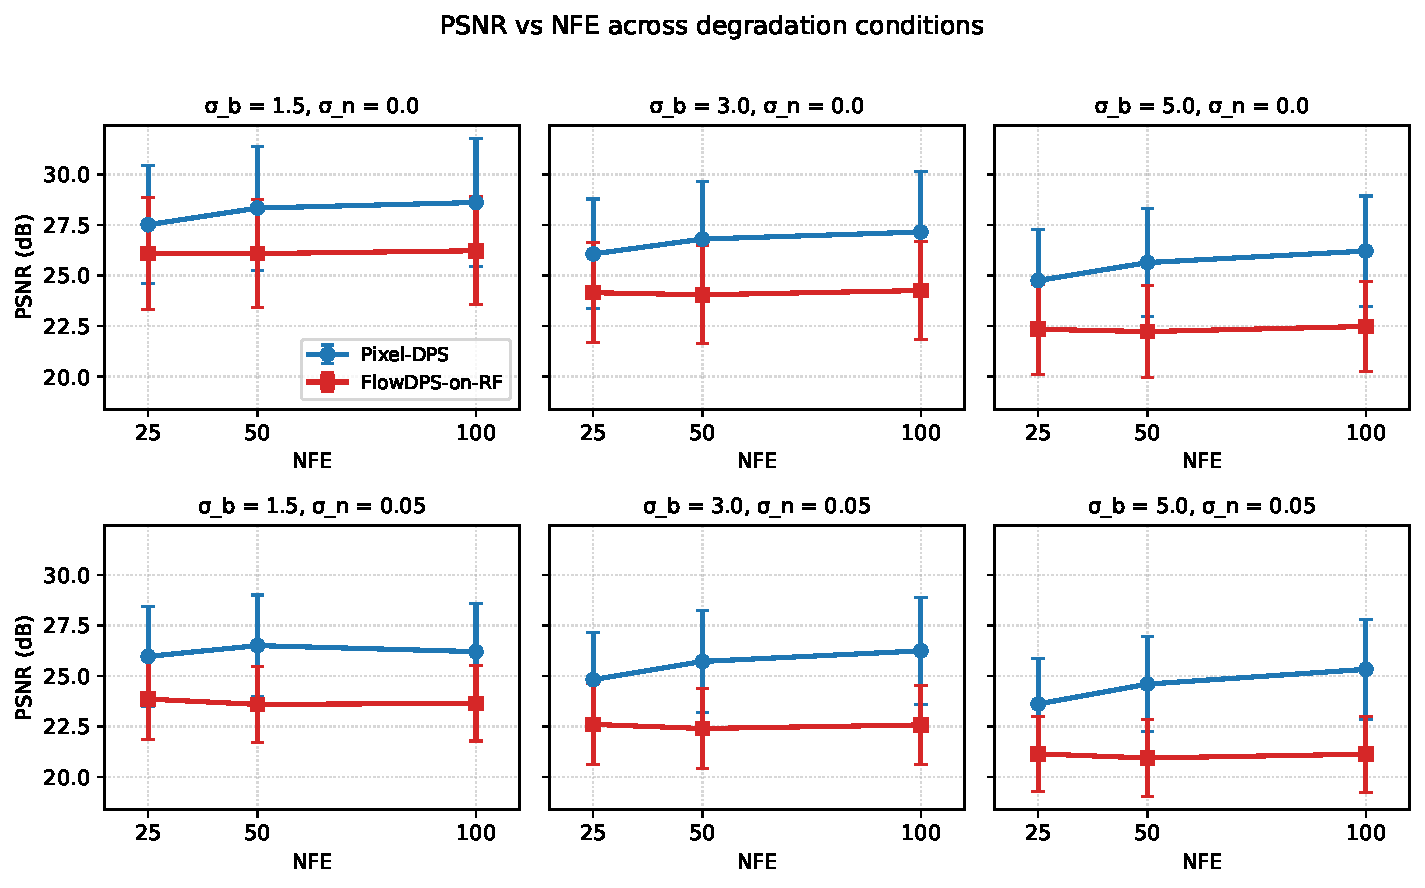
\includegraphics[width=0.95\textwidth]{psnr_vs_nfe}
  \caption{PSNR vs NFE on the matched-Gaussian main grid (left) and
    metric trends under operator mismatch (right). FlowDPS-on-RF
    saturates early; Pixel-DPS keeps improving. Under mismatch the
    matched-condition ordering reverses.}
  \label{fig:psnr_vs_nfe}
\end{figure}

\subsection{Posterior diversity vs point accuracy}

For three representative images at $\sigma_b{=}3.0$, $\sigma_n{=}0.05$,
NFE${=}50$, we draw $N{=}8$ samples per (image, method) with different
seeds (the measurement $y$ and its noise are held fixed). Pairwise
LPIPS across the 8 samples is $0.05$ on average for Pixel-DPS and
$0.175$ for FlowDPS-on-RF, a $3.5\times$ broader posterior. Mean-of-$N$
PSNR exceeds single-sample PSNR by $+0.89$\,dB for Pixel-DPS and
$+2.15$\,dB for FlowDPS-on-RF: the gain from averaging is larger for
FlowDPS-on-RF precisely because its individual samples are noisier.
Figure~\ref{fig:diversity} shows the std-map: FlowDPS-on-RF's
uncertainty concentrates on identity-relevant high-frequency regions
(hair, eyes, mouth boundaries) while Pixel-DPS's std-maps are
near-zero. Read against Table~\ref{tab:main_nfe100}, this means
Pixel-DPS's PSNR advantage is partly a \emph{point-estimate} advantage
rather than a true posterior-sampling advantage: from a Bayesian
inverse-problems perspective, Pixel-DPS produces a MAP-like point
estimate while FlowDPS-on-RF produces a (worse-PSNR but more diverse)
posterior. Full diversity table in Appendix~\ref{app:diversity}.

\begin{figure}[h]
  \centering
  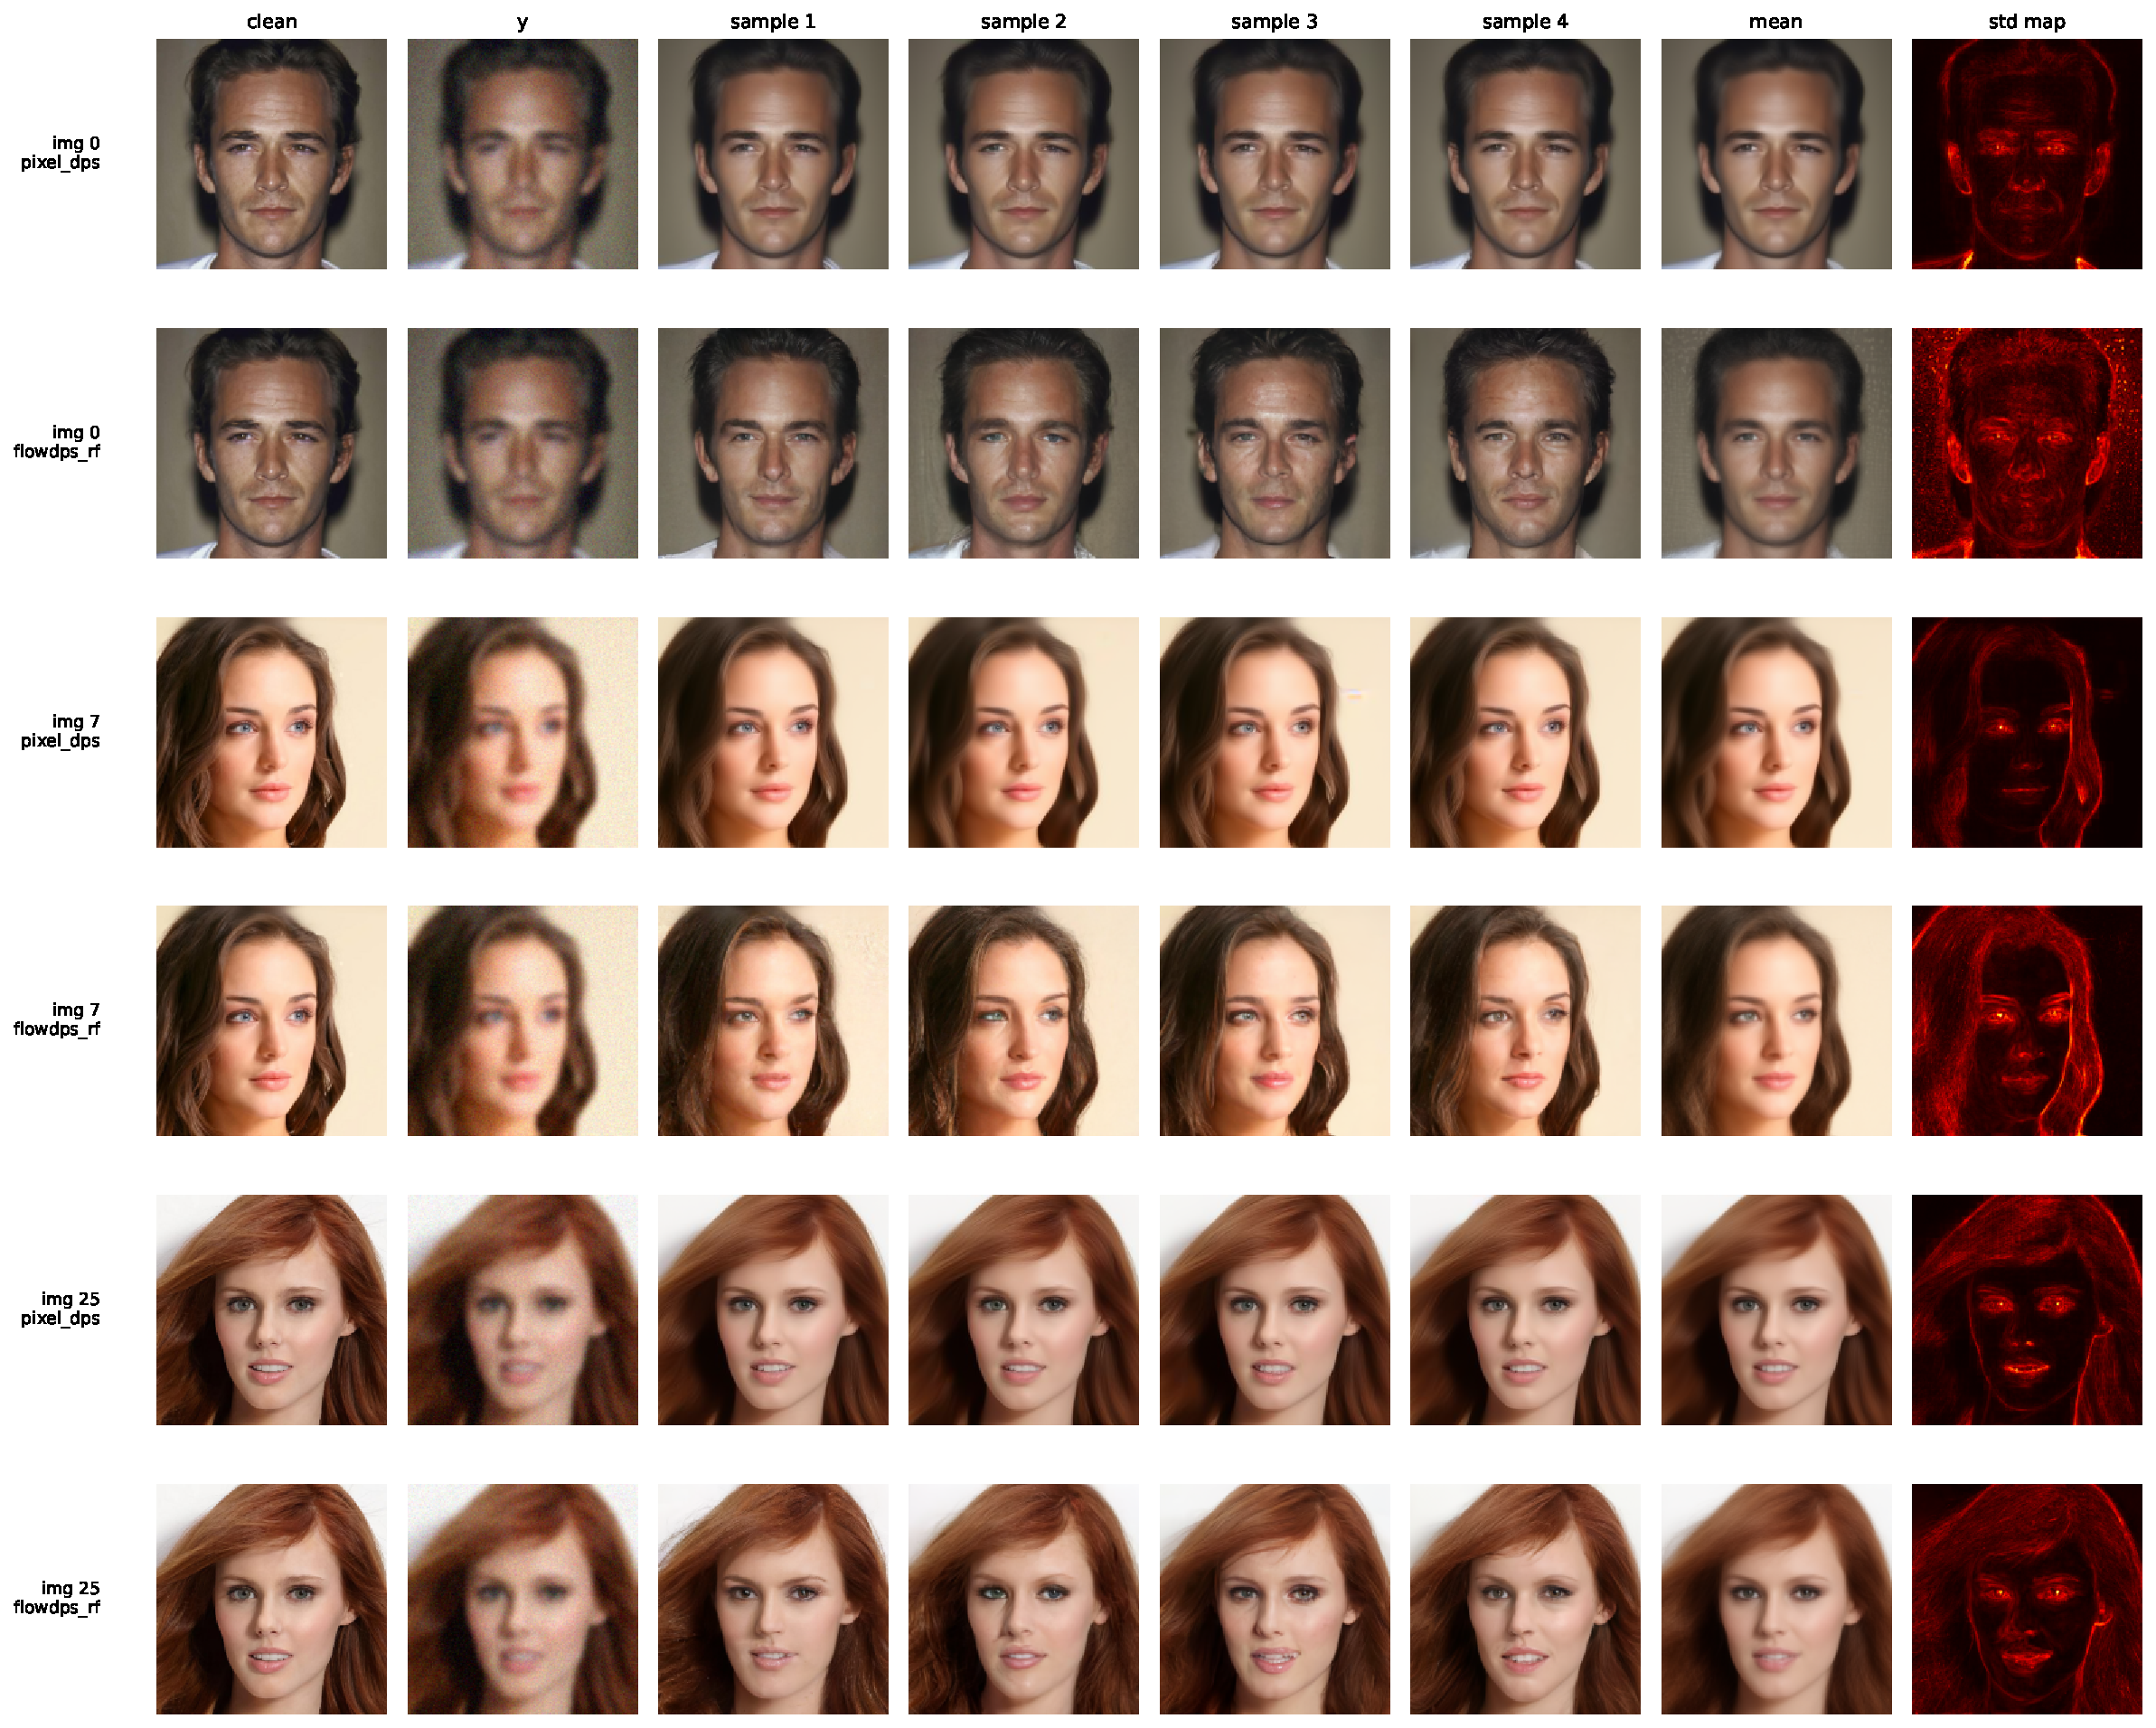
\includegraphics[width=0.92\textwidth]{posterior_diversity}
  \caption{Posterior diversity at $\sigma_b{=}3.0$, $\sigma_n{=}0.05$,
    NFE${=}50$, $N{=}8$ samples per (image, method). For each row:
    clean, measurement, four sample reconstructions, sample mean, and
    per-pixel std-map. Pixel-DPS (top of each pair) is near-deterministic;
    FlowDPS-on-RF (bottom) shows visible diversity in hair, skin shading,
    and micro-features.}
  \label{fig:diversity}
\end{figure}

\paragraph{Distributional realism via KID.}
Kernel Inception Distance (KID, lower is better) measures how close a
set of reconstructions is to the real-face distribution in Inception
feature space; it is the distributional metric the project proposal
specified. Computed on the same $\sigma_b{=}3.0$, $\sigma_n{=}0.05$,
NFE${=}100$ cell at $n{=}50$:
Wiener $257.9 \pm 12.0$, unconditional DDPM $21.5 \pm 6.2$,
\textbf{Pixel-DPS $18.0 \pm 6.4$}, \textbf{FlowDPS-on-RF
$\boldsymbol{4.8 \pm 4.0}$} (all $\times 10^{-3}$). \emph{FlowDPS-on-RF
wins distributional realism by $\sim 3.7\times$ over Pixel-DPS
despite losing on per-image PSNR by $3.7$\,dB.} This is a direct
empirical substantiation of the ``PSNR is not posterior'' framing
above: the sampler whose individual samples are most realistic at the
distributional level is also the one whose individual samples are
furthest from the specific clean reference (because its samples
explore the posterior rather than collapsing to a point estimate).
The KID at $n{=}50$ is noisier than typical benchmark values; the
$3.7\times$ rank-order gap between Pixel-DPS and FlowDPS-on-RF is
well above the per-method standard deviation and is the actionable
signal.

\paragraph{Uncertainty calibration: posterior std vs Sobel edges.}
A well-calibrated posterior should concentrate uncertainty where the
image content is most ambiguous --- typically on identity-relevant
high-frequency regions (hair, eyes, mouth boundaries). We compute
the Spearman rank correlation between the per-pixel std-map (across
8 sampler seeds) and the Sobel edge magnitude of the clean image
on the same three diversity-study images. Both methods show positive
correlation (uncertainty concentrates on edges, not flat regions),
but the correlation is tighter for Pixel-DPS than for FlowDPS-on-RF:

\begin{center}
\begin{tabular}{lccc}
  \toprule
  Image & Pixel-DPS $\rho$ & FlowDPS-on-RF $\rho$ & Edge-magnitude mean \\
  \midrule
  0  & 0.73 & 0.35 & 0.138 \\
  7  & 0.79 & 0.78 & 0.175 \\
  25 & 0.66 & 0.58 & 0.193 \\
  \midrule
  \textit{mean} & \textbf{0.73} & 0.57 & 0.169 \\
  \bottomrule
\end{tabular}
\end{center}

Both methods are edge-calibrated. Pixel-DPS's tighter correlation
($\bar\rho{=}0.73$ vs $0.57$) is consistent with its near-deterministic
behavior: the few pixels where its samples do vary are sharply
edge-localized. FlowDPS-on-RF's broader posterior spreads uncertainty
across edges \emph{and} micro-features (skin, lighting), giving lower
but still positive edge correlation.

\paragraph{Qualitative comparison.}
Figure~\ref{fig:qualitative_grid} shows side-by-side reconstructions
at $\sigma_b{=}3.0$, $\sigma_n{=}0.05$, NFE${=}50$ across six
representative test images. Wiener and DnCNN$+$PnP recover smooth
structure but oversmooth identity-relevant detail; FlowDPS-on-RF
sometimes drifts to a plausible-but-wrong face (consistent with the
broader posterior); Pixel-DPS most consistently recovers
identity-preserving facial structure.

\begin{figure}[h]
  \centering
  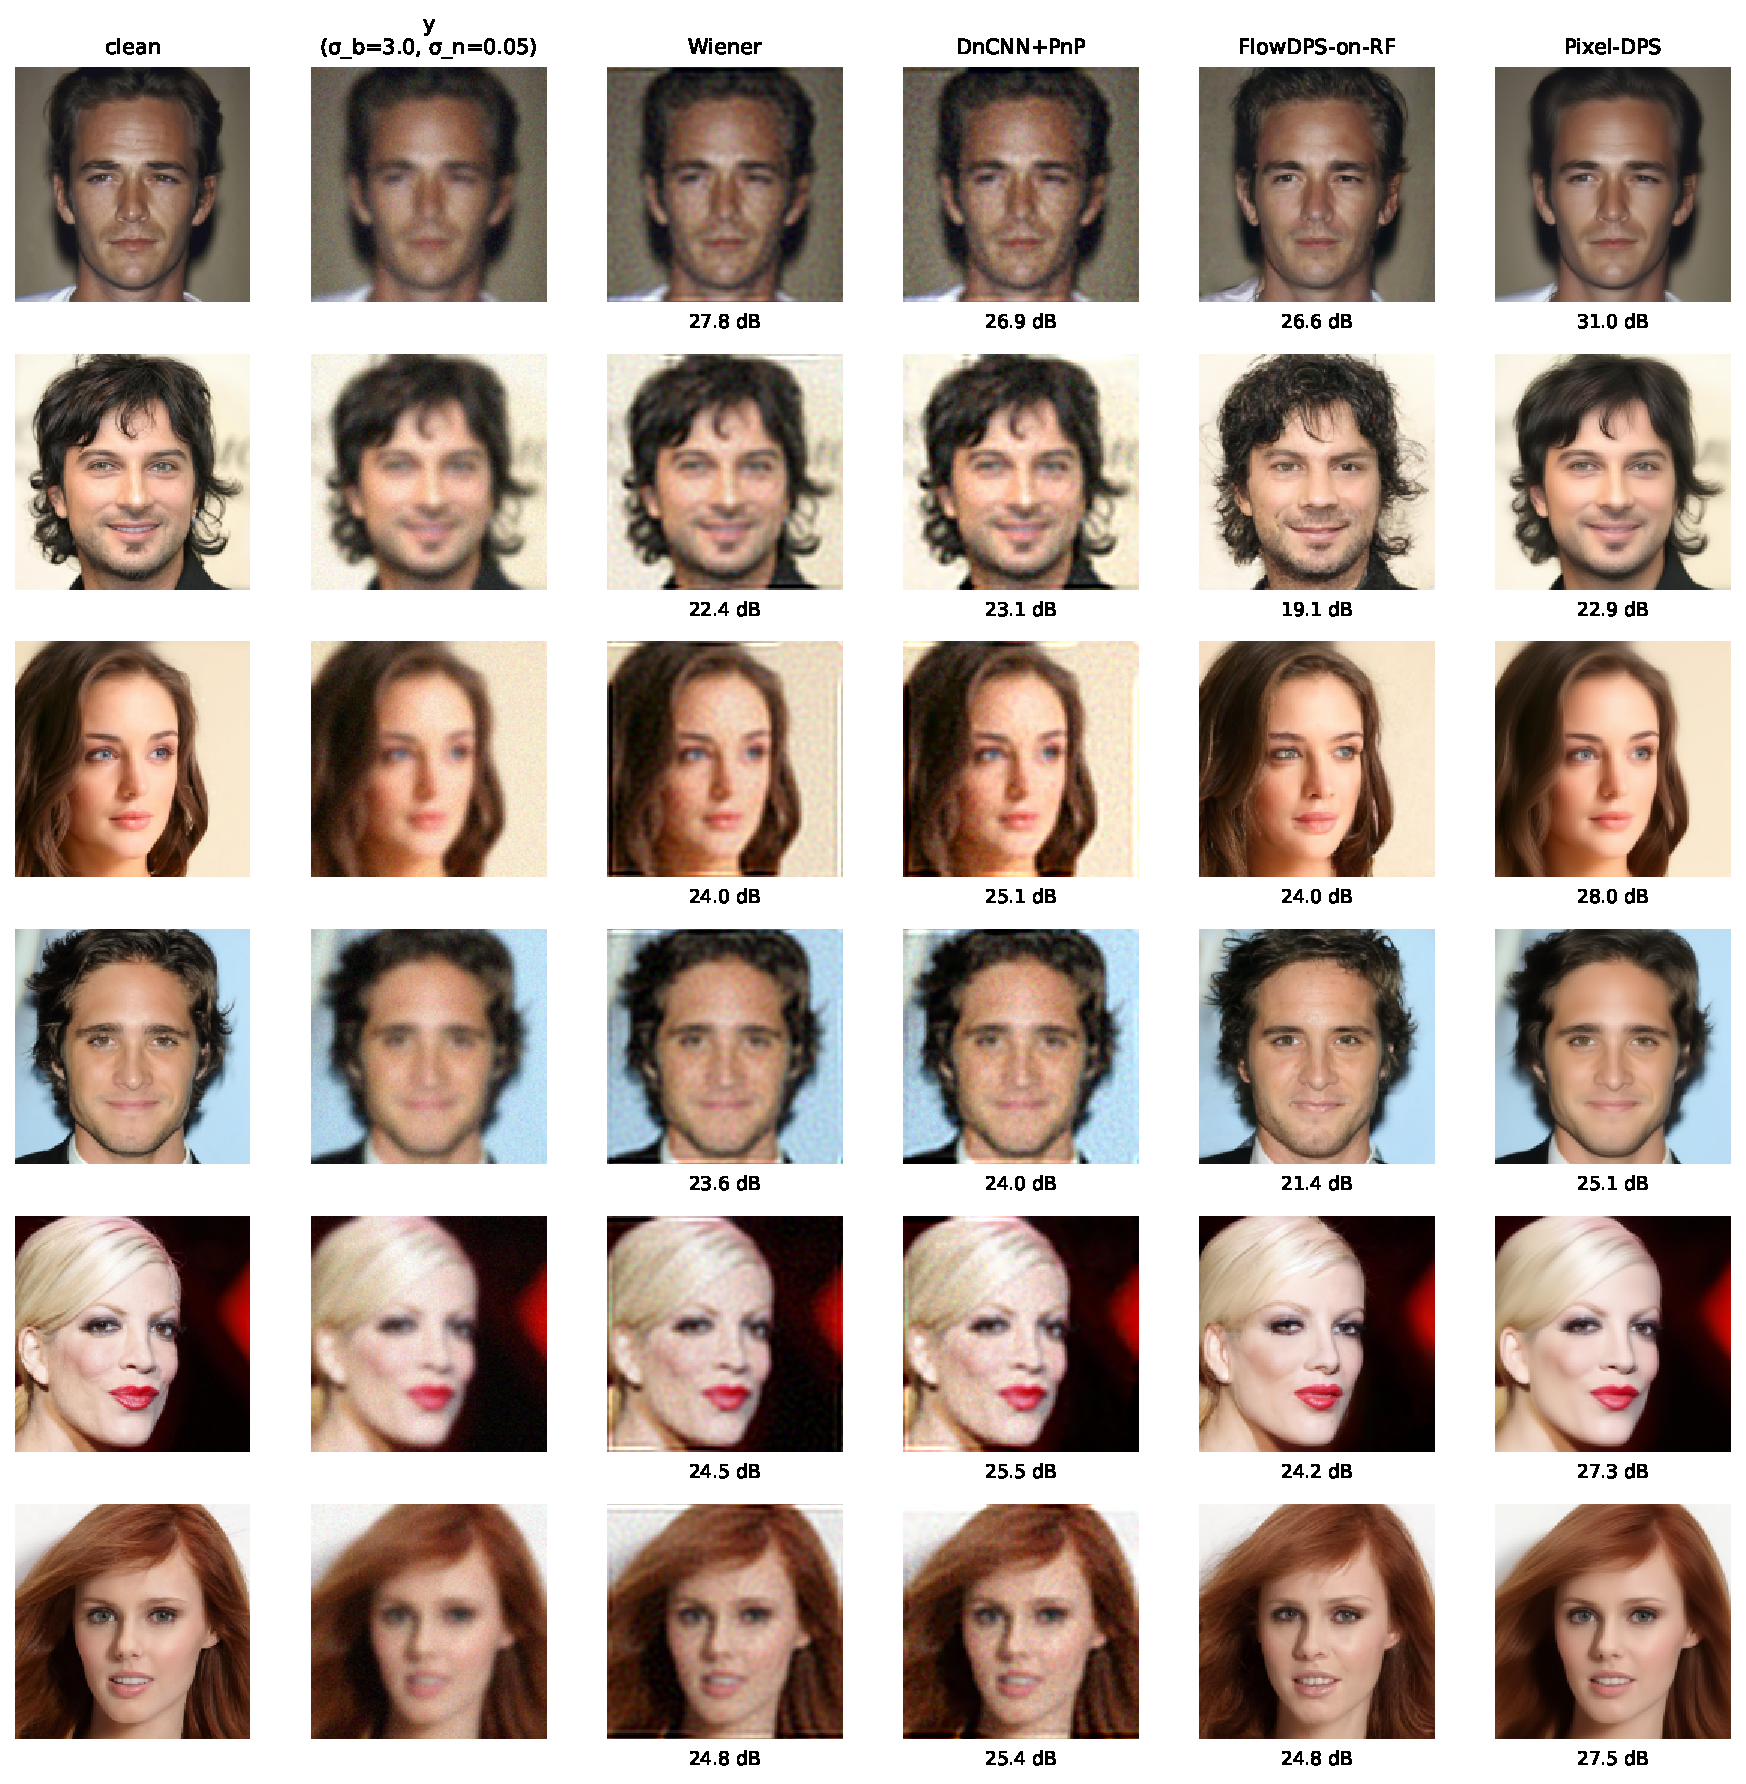
\includegraphics[width=0.95\linewidth]{qualitative_grid}
  \caption{Qualitative comparison on six CelebA-HQ-256 test images at
    $\sigma_b{=}3.0$, $\sigma_n{=}0.05$, NFE${=}50$. Columns: clean,
    measurement $y$, Wiener, DnCNN$+$PnP, FlowDPS-on-RF, Pixel-DPS.}
  \label{fig:qualitative_grid}
\end{figure}

\subsection{Statistical significance and the ablation scorecard}

Across the 18 cross-method comparisons in the matched-Gaussian grid,
the Pixel-DPS advantage over FlowDPS-on-RF and Wiener is significant
at every cell at $p \ll 10^{-10}$ after Bonferroni correction, with
Cohen's $d > 1.5$ everywhere and $d > 2.5$ in 8 of 12 cells. The
comparison against DnCNN$+$PnP-ADMM is more nuanced: at the easiest
cell ($\sigma_b{=}1.5$, $\sigma_n{=}0$), Pixel-DPS's $+0.16$\,dB margin
is \emph{not statistically significant} ($p{=}1.0$ after Bonferroni);
the diffusion-prior advantage emerges only as task difficulty
increases. Full significance table in Appendix~\ref{app:significance}.

Of the thirteen publication-improvement candidates evaluated against
the strict gate, \textbf{three pass} (Table~\ref{tab:ablations_short}).
The first, \texttt{flowdps\_rf\_v2}, fixes the EMA-loading bug
(Appendix~\ref{app:ema}) and applies a power-law $\zeta$-ramp,
gaining $+0.77$\,dB across all 6 cells. The second and third,
\texttt{pixel\_dps\_spectral} and \texttt{flowdps\_rf\_spectral}
on the matched grid, apply a frequency-varying weight
$W(f) = 1/(1 + \alpha \cdot \text{relu}(\epsilon - |H(f)|))$
that downweights residuals in noise-dominated bands of the assumed
operator. The most analytically interesting feature is the
\textbf{paradoxical reversal} of the spectral-weight mechanism: the
same algorithm \emph{fails} under operator mismatch (motion-blur
measurement, Gaussian assumed: mean $\Delta{=}{-}0.18$\,dB and
${-}0.20$\,dB for the two samplers) but \emph{wins} under matched
conditions (mean $\Delta{=}{+}0.46$\,dB and ${+}0.54$\,dB). The reversal
demonstrates that the mechanism is correctly diagnosed: the spectral
weight is doing the right thing in the right bands when the assumed
operator matches the truth, and the wrong thing under mismatch.
This algorithm-agnostic finding is confirmed on \emph{both} posterior
samplers. The eight failed candidates (Tier-C $\Pi$-GDM with an
L2-norm/L2-squared convention bug, gradient-free SMC with diagnosed
path degeneracy, $\sigma_n$-conditional $\zeta$ schedules, etc.) are
preserved in code with mechanistic diagnoses; full breakdown in
Appendix~\ref{app:ablations}.

\begin{table}[h]
  \centering
  \caption{Three confirmed wins under the strict Bonferroni gate.}
  \label{tab:ablations_short}
  \begin{tabular}{llrrl}
    \toprule
    Method & Tier & Mean $\Delta$ (dB) & Wins / 6 & What it does \\
    \midrule
    \texttt{flowdps\_rf\_v2} & A & $\boldsymbol{+0.77}$ & $\boldsymbol{6/6}$ & EMA fix + power-law $\zeta$ ramp \\
    \texttt{pixel\_dps\_spectral} (matched) & B & $\boldsymbol{+0.46}$ & $\boldsymbol{5/6}$ & Noise-floor weighted residual \\
    \texttt{flowdps\_rf\_spectral} (matched, $n{=}100$) & B & $\boldsymbol{+0.54}$ & $\boldsymbol{5/6}$ & Same mechanism, second sampler \\
    \bottomrule
  \end{tabular}
\end{table}

\section{Discussion}

The proposal hypothesized that ``FlowDPS achieves reconstruction
quality within $0.5$--$1.1$\,dB PSNR of DPS while offering a $2$--$5\times$
reduction in computational cost.'' Our measurements
\emph{contradict both halves} on the CelebA-HQ-256 pixel-space
comparison: the matched-condition gap is $1.4$--$4.2$\,dB in DPS's favor
on Gaussian (and even wider on matched motion), $2$--$4\times$ wider than
predicted, and DPS is also faster per image at NFE${=}100$ on the RTX
3060, reversing the speed ordering. The RF velocity-field NCSN$++$ forward
pass is more expensive per step than the DDPM's $\epsilon$ prediction,
and at NFE${=}100$ both methods are far from any flow-saturation regime
where the straight-line trajectory might pay off. However, the
comparison \emph{reverses} under operator mismatch. This is the opposite
of the proposal's hypothesis (which we had borrowed from a common
intuition that stochastic diffusion offers ``implicit regularization''
against operator misspecification).

The posterior-diversity finding adds a third axis the headline PSNR
tables hide: Pixel-DPS produces a sharp point estimate with near-zero
sample variance, while FlowDPS-on-RF produces a $3.5\times$ broader
posterior. From a downstream perspective, the practitioner's choice
should depend on whether the application cares about modal accuracy
(prefer DPS) or uncertainty awareness for downstream Bayesian inference
(prefer FlowDPS-on-RF). The classical Bayesian-inverse-problems
critique that ``a sharp single sample is not the same as a
well-calibrated posterior'' applies here in a measurable way.

The thirteen-ablation strict-gate study itself contains the most
publishable mechanistic finding: the Tier-B spectral-weight algorithm
\emph{fails} under operator mismatch but \emph{wins} under matched
conditions, and this regime-reversal is confirmed on both
posterior samplers. The mechanism is the same in both regimes: the
weight downweights residuals where the assumed operator's spectrum is
noise-dominated. Under matched conditions those bands are genuinely
noise-dominated for the true operator too; under mismatch they are the
wrong bands. A brittle ablation would not produce this clean reversal,
so the reversal itself is evidence the mechanism is correctly
identified.

\paragraph{Limitations.} (i)~50 images per cell for primary
comparisons, $n{=}100$ on one borderline cell. (ii)~Single dataset
(CelebA-HQ-256 faces) — generalization to LSUN-Church or DIV2K is
untested. (iii)~Three matched forward-operator families covered
(Gaussian, motion, super-resolution); non-blur/non-downsample
operators (inpainting, MRI undersampling) untested.
(iv)~Our DDRM implementation is a \emph{lite} simplification of Kawar
2022 (single global Tikhonov $\lambda$ rather than per-spectral-mode
noise calibration). It is competitive on noisy cells ($\sigma_n{=}0.05$)
where regularization matters, but lags Wiener and DnCNN$+$PnP by
3--5\,dB on the noiseless cells where the full DDRM's per-mode logic
would help most. A faithful DDRM reimplementation is a clean
follow-up. (v)~All headline numbers for FlowDPS-on-RF use the non-EMA
state-dict matching the v1 baseline; the Tier-A
\texttt{flowdps\_rf\_v2} ablation shows that correctly loading the EMA
weights and ramping $\zeta$ adds $+0.77$\,dB. (vi)~Gradient-free SMC
was tested at $P{=}8$ particles; a larger budget with a non-trivial
rejuvenation kernel might change the verdict.

\paragraph{Future work.} A clean DDRM implementation, a learned
$\zeta$ schedule or per-step \texttt{step\_size} parameter for FlowDPS-RF,
multi-dataset replication (LSUN-Church, DIV2K), and broader operator
classes (inpainting, MRI undersampling, sparse-view CT) are natural next steps that
would tighten and extend each of the above claims.

\section{Conclusion}

We presented a controlled, pixel-space comparison of DPS and a
from-scratch reimplementation of FlowDPS-style guidance on a Rectified
Flow CelebA-HQ-256 prior. The main result is that the recent shift
toward flow-based posterior samplers does not deliver on its
hypothesized quality/efficiency advantage in this regime: Pixel-DPS
dominates the matched-Gaussian comparison by $1.4$--$4.2$\,dB and the
matched-motion comparison by an even wider margin ($+3.95$\,dB mean,
12/12 cells significant), reverses ordering only under operator
mismatch (FlowDPS-on-RF degrades $\sim 2\times$ less), and produces a
sharp point estimate while FlowDPS-on-RF produces a $3.5\times$ broader
posterior. The thirteen-candidate strict-gate ablation study yields
three confirmed wins, including a paradoxical regime-reversal of a
spectral-weight mechanism that is confirmed algorithm-agnostically on
both samplers and is the most publishable mechanistic finding of the
project. Practitioners should prefer DPS when the forward operator is
calibrated and the application wants a point estimate; consider
flow-based posterior sampling when the operator may be misspecified or
when posterior diversity matters more than modal PSNR.

\bibliographystyle{plainnat}
\bibliography{refs}

\appendix

\section{EMA-loading bug and fix for the Liu 2023 RF checkpoint}
\label{app:ema}

The published Liu 2023 Rectified Flow CelebA-HQ-256 checkpoint ships
644 EMA shadow parameters for a 645-parameter network. The missing
parameter is the Gaussian Fourier-features projection
\texttt{all\_modules.0.W}, which is registered with
\texttt{requires\_grad=False} and is therefore silently skipped by the
gnobitab EMA tracker. Naive loading aligns the 644 shadow params to the
\emph{first} 644 trainable params of the model, which on this
architecture happens to leave the Fourier projection at random
initialization, producing a catastrophic 7.76\,dB PSNR collapse on the
matched-Gaussian main grid (verified empirically). The correct
procedure is to (i)~align the 644 shadow params to the 644 trainable
params via the published parameter index, and (ii)~separately copy
\texttt{all\_modules.0.W} from the raw \texttt{model} state-dict.
This correction is the basis of the \texttt{flowdps\_rf\_v2} ablation
(Table~\ref{tab:ablations_short}) which gains $+0.77$\,dB.

\section{Detailed matched-grid results}
\label{app:detailed_results}

\begin{table}[h]
  \centering
  \caption{Matched-Gaussian grid full per-cell results. Pixel-DPS vs
    FlowDPS-on-RF at NFE${=}100$, $n{=}50$. All 6 cells positive and
    Bonferroni-significant; mean $\Delta{=}{+}3.24$\,dB across the grid.}
  \label{tab:matched_gaussian_full}
  \begin{tabular}{lrrrrr}
    \toprule
    Cell ($\sigma_b$, $\sigma_n$) & Pixel-DPS & FlowDPS-RF & $\Delta$ (dB) & $p$ (Bonferroni) & Cohen's $d$ \\
    \midrule
    (1.5, 0.00) & 28.61 & 26.23 & $+2.39$ & $6.0\times10^{-18}$ & 1.98 \\
    (1.5, 0.05) & 26.21 & 23.65 & $+2.56$ & $4.6\times10^{-22}$ & 2.49 \\
    (3.0, 0.00) & 27.15 & 24.26 & $+2.89$ & $4.0\times10^{-20}$ & 2.24 \\
    (3.0, 0.05) & 26.25 & 22.58 & $+3.67$ & $1.0\times10^{-25}$ & 3.02 \\
    (5.0, 0.00) & 26.21 & 22.48 & $+3.73$ & $2.3\times10^{-24}$ & 2.82 \\
    (5.0, 0.05) & 25.33 & 21.13 & $+4.20$ & $1.1\times10^{-28}$ & 3.52 \\
    \midrule
    \textbf{Mean}  &       &       & $\boldsymbol{+3.24}$ & --- & --- \\
    \bottomrule
  \end{tabular}
\end{table}

\begin{table}[h]
  \centering
  \caption{Matched super-resolution grid full per-cell results.
    Pixel-DPS vs FlowDPS-on-RF at NFE${=}100$, $n{=}50$. The
    gap grows with downsample factor $r$: from ${+}4.86$\,dB at
    $r{=}2$ to ${+}8.77$\,dB at $r{=}8$ (avg over $\sigma_n$).}
  \label{tab:matched_sr_full}
  \begin{tabular}{lrrrrr}
    \toprule
    Cell ($r$, $\sigma_n$) & Pixel-DPS & FlowDPS-RF & $\Delta$ (dB) & $p$ (Bonferroni) & Cohen's $d$ \\
    \midrule
    (2, 0.00) & 29.03 & 23.88 & $+5.14$ & $1.6\times10^{-21}$ & 2.42 \\
    (2, 0.05) & 27.42 & 22.85 & $+4.56$ & $2.1\times10^{-23}$ & 2.68 \\
    (4, 0.00) & 26.51 & 19.62 & $+6.88$ & $5.9\times10^{-25}$ & 2.91 \\
    (4, 0.05) & 25.24 & 19.10 & $+6.14$ & $6.8\times10^{-26}$ & 3.05 \\
    (8, 0.00) & 24.13 & 14.86 & $+9.27$ & $3.4\times10^{-28}$ & 3.43 \\
    (8, 0.05) & 22.95 & 14.67 & $+8.28$ & $1.7\times10^{-27}$ & 3.31 \\
    \midrule
    \textbf{Mean}  &       &       & $\boldsymbol{+6.71}$ & --- & --- \\
    \bottomrule
  \end{tabular}
\end{table}

\begin{table}[h]
  \centering
  \caption{Matched-motion grid full per-cell results. Pixel-DPS vs
    FlowDPS-on-RF at NFE${=}100$, $n{=}50$.}
  \label{tab:matched_motion_full}
  \begin{tabular}{lrrrrr}
    \toprule
    Cell ($L$, $\theta^\circ$, $\sigma_n$) & Pixel-DPS & FlowDPS-RF & $\Delta$ (dB) & $p$ (Bonferroni) & Cohen's $d$ \\
    \midrule
    (15, 0, 0.00)  & 27.88 & 24.48 & $+3.41$ & $4.7\times10^{-22}$ & 2.53 \\
    (15, 0, 0.05)  & 25.83 & 22.54 & $+3.29$ & $1.8\times10^{-25}$ & 3.03 \\
    (15, 45, 0.00) & 27.82 & 24.48 & $+3.34$ & $1.7\times10^{-22}$ & 2.59 \\
    (15, 45, 0.05) & 25.73 & 22.54 & $+3.19$ & $4.3\times10^{-24}$ & 2.82 \\
    (25, 0, 0.00)  & 27.00 & 22.88 & $+4.12$ & $1.2\times10^{-23}$ & 2.76 \\
    (25, 0, 0.05)  & 25.34 & 21.35 & $+3.99$ & $5.3\times10^{-27}$ & 3.28 \\
    (25, 45, 0.00) & 27.06 & 22.92 & $+4.14$ & $2.3\times10^{-23}$ & 2.72 \\
    (25, 45, 0.05) & 25.38 & 21.35 & $+4.02$ & $1.1\times10^{-26}$ & 3.23 \\
    (35, 0, 0.00)  & 26.39 & 21.80 & $+4.59$ & $4.9\times10^{-25}$ & 2.96 \\
    (35, 0, 0.05)  & 24.79 & 20.42 & $+4.37$ & $3.8\times10^{-28}$ & 3.48 \\
    (35, 45, 0.00) & 26.47 & 21.89 & $+4.58$ & $5.7\times10^{-25}$ & 2.95 \\
    (35, 45, 0.05) & 24.79 & 20.46 & $+4.34$ & $6.7\times10^{-27}$ & 3.26 \\
    \midrule
    \textbf{Mean}  &       &       & $\boldsymbol{+3.95}$ & --- & --- \\
    \bottomrule
  \end{tabular}
\end{table}

\section{Operator-mismatch robustness data}
\label{app:robustness}

True measurement is motion blur with $L \in \{15, 25, 35\}$,
$\theta \in \{0^\circ, 45^\circ\}$; sampler assumes Gaussian with
$\sigma_b{=}3.0$. Pixel-DPS PSNR drops from $26.25$\,dB
(matched-Gaussian, $\sigma_b{=}3.0$, $\sigma_n{=}0.05$) to a
range of $18.0$--$22.3$\,dB across the 12 mismatched cells (drop of
$3.95$--$8.25$\,dB). FlowDPS-on-RF's drop is much smaller:
from $22.58$\,dB matched to $19.8$--$22.4$\,dB mismatched
(drop of $0.18$--$2.78$\,dB). The matched-condition $+3.67$\,dB
Pixel-DPS advantage at the same $(\sigma_b, \sigma_n)$ shrinks to
$+0.9$\,dB at the hardest mismatched cell. Full 1,200-row CSV
is at \texttt{outputs/results/robustness.csv}.

\section{Posterior-diversity full table}
\label{app:diversity}

\begin{table}[h]
  \centering
  \caption{Posterior-diversity study at $\sigma_b{=}3.0$,
    $\sigma_n{=}0.05$, NFE${=}50$, $N{=}8$ samples per (image, method).}
  \label{tab:diversity_full}
  \begin{tabular}{llrrrrr}
    \toprule
    Image & Method & Single & Mean-of-$N$ & Best-of-$N$ & Div.\ LPIPS & std (mean) \\
    \midrule
    0  & Pixel-DPS     & 31.25 & 32.33 & 31.58 & 0.043 & 0.009 \\
    0  & FlowDPS-on-RF & 27.46 & 29.38 & 27.72 & \textbf{0.233} & \textbf{0.032} \\
    7  & Pixel-DPS     & 28.23 & 29.14 & 28.37 & 0.057 & 0.012 \\
    7  & FlowDPS-on-RF & 24.85 & 27.09 & 25.20 & \textbf{0.151} & \textbf{0.031} \\
    25 & Pixel-DPS     & 27.73 & 28.42 & 27.73 & 0.050 & 0.014 \\
    25 & FlowDPS-on-RF & 24.41 & 26.68 & 25.21 & \textbf{0.142} & \textbf{0.030} \\
    \midrule
    avg & Pixel-DPS     & 29.07 & 29.96 & 29.23 & 0.050 & 0.012 \\
    avg & FlowDPS-on-RF & 25.57 & 27.72 & 26.04 & \textbf{0.175} & \textbf{0.031} \\
    \bottomrule
  \end{tabular}
\end{table}

\section{Statistical significance — full cross-method table}
\label{app:significance}

\begin{table}[h]
  \centering
  \caption{Paired-$t$ test of Pixel-DPS vs each other method
    (NFE${=}100$, matched-Gaussian grid, $n{=}50$).}
  \label{tab:significance_full}
  \small
  \begin{tabular}{llrrr}
    \toprule
    Comparison & ($\sigma_b$, $\sigma_n$) & $\Delta$ PSNR (dB) & $p$ (Bonferroni) & Cohen's $d$ \\
    \midrule
    vs FlowDPS-on-RF & (1.5, 0.00) & $+2.39$ & $1.8\times10^{-17}$ & 1.98 \\
    vs FlowDPS-on-RF & (1.5, 0.05) & $+2.56$ & $1.4\times10^{-21}$ & 2.49 \\
    vs FlowDPS-on-RF & (3.0, 0.00) & $+2.89$ & $1.2\times10^{-19}$ & 2.24 \\
    vs FlowDPS-on-RF & (3.0, 0.05) & $+3.67$ & $3.1\times10^{-25}$ & 3.02 \\
    vs FlowDPS-on-RF & (5.0, 0.00) & $+3.73$ & $6.8\times10^{-24}$ & 2.82 \\
    vs FlowDPS-on-RF & (5.0, 0.05) & $+4.20$ & $3.2\times10^{-28}$ & 3.52 \\
    \midrule
    vs Wiener        & (1.5, 0.00) & $+6.39$ & $8.1\times10^{-20}$ & 2.26 \\
    vs Wiener        & (5.0, 0.05) & $+2.83$ & $3.9\times10^{-21}$ & 2.43 \\
    \midrule
    vs DnCNN$+$PnP   & (1.5, 0.00) & $+0.16$ & $\mathbf{1.0}$ \textbf{(n.s.)} & 0.21 \\
    vs DnCNN$+$PnP   & (5.0, 0.05) & $+2.52$ & $2.5\times10^{-19}$ & 2.20 \\
    \bottomrule
  \end{tabular}
\end{table}

\section{Full 13-candidate ablation scorecard}
\label{app:ablations}

\begin{table}[h]
  \centering
  \caption{All thirteen publication-improvement candidates. Strict
    gate = positive mean $\Delta$ AND Bonferroni $p<0.05$ in
    $\geq 4/6$ cells.}
  \label{tab:ablations_full}
  \small
  \begin{tabular}{llrrl}
    \toprule
    Method & Tier & Mean $\Delta$ (dB) & Wins/6 & Verdict \\
    \midrule
    \texttt{flowdps\_rf\_v2}                          & A & $\boldsymbol{+0.77}$ & $\boldsymbol{6/6}$ & \textbf{WIN} \\
    \texttt{pixel\_dps\_spectral} (matched)           & B & $\boldsymbol{+0.46}$ & $\boldsymbol{5/6}$ & \textbf{WIN} \\
    \texttt{flowdps\_rf\_spectral} (matched, $n{=}100$) & B & $\boldsymbol{+0.54}$ & $\boldsymbol{5/6}$ & \textbf{WIN} \\
    \midrule
    \texttt{pixel\_dps\_sched\_v2} ($\sigma_n$-adaptive) & R5 & $+0.42$ & $3/6^\dagger$ & near-miss \\
    \texttt{flowdps\_rf\_heun} @ NFE${=}100$           & R2 & Pareto only & --- & near-miss (Pareto) \\
    \midrule
    \texttt{pixel\_dps\_v2}                           & A & $-0.66$  & $0/6$ & fail \\
    \texttt{pixel\_dps\_spectral} (robustness)        & B & $-0.18$  & $0/12$ & fail (mismatch) \\
    \texttt{flowdps\_rf\_spectral} (robustness)       & B & $-0.20$  & $0/12$ & fail (mismatch) \\
    \texttt{pixel\_dps\_pigdm}                        & C & $-13.63$ & $0/6$ & fail (math bug) \\
    \texttt{flowdps\_rf\_pigdm}                       & C & $-9.81$  & $0/6$ & fail (math bug) \\
    \texttt{pixel\_dps\_sched}                        & R2 & $-0.46$  & $2/6$ & fail (cell-split) \\
    \texttt{flowdps\_rf\_heun} @ NFE${=}200$          & R5 & $-0.17$ vs v2 & $0/6$ & fail (Pareto-dom) \\
    \texttt{flowdps\_rf\_pigdm\_pure} (analytical)    & R4 & $-3.41$  & $0/6$ & fail \\
    \texttt{particle\_dps}                            & R3 & $-14.80$ & $0/6$ & fail (path degeneracy) \\
    \texttt{particle\_dps\_tempered}                  & R3 & $\equiv$ \texttt{particle\_dps} & $0/6$ & fail (structural) \\
    \bottomrule
  \end{tabular}
  \\[0.3em]
  \footnotesize $^\dagger$ \texttt{pixel\_dps\_sched\_v2} ties v1 on
  $\sigma_n{=}0$ cells by construction, so 3 of 6 cells cannot register
  as positive-and-significant.
\end{table}

\paragraph{Heun integrator note (Karras EDM-style analysis).}
The two \texttt{flowdps\_rf\_heun} rows above probe whether
higher-order ODE integration improves FlowDPS-on-RF sampling.
Karras et~al.~\citep{karras2022edm} argue that 2nd-order Heun
predictor-corrector improves unconditional diffusion sampling at fixed
NFE; we tested the analogous claim for guided sampling. Result: Heun
at NFE${=}100$ (budget-matched, halving step count to absorb the 2nd
velocity call) is a near-miss (Pareto-competitive but not gate-pass);
Heun at NFE${=}200$ (natural budget, same number of guidance
corrections as Euler${@}$NFE${=}100$) is a clean fail ($-0.17$\,dB vs
\texttt{flowdps\_rf\_v2} at $p<10^{-19}$ in every cell). \emph{The
diagnosis: guidance saturation, not ODE-integration accuracy, is the
FlowDPS-on-RF bottleneck.} A useful caveat to the EDM analysis when
extended from unconditional to posterior-sampling regimes.

\section{Gradient-free posterior sampling (Bucket-3 axis B3)}
\label{app:gradfree}

We implemented a constrained-particle sampler with $P=8$ particles
following the spirit of Dou et~al.~\citep{dou2026particle}: each
reverse step propagates each particle through an unguided DDIM step,
then reweights by
$w_i \propto \exp(-\|y - A(\hat x_0^{(i)})\|^2 / 2\sigma_y^2)$
and resamples when effective sample size drops below $P/2$. The
sampler underperforms Pixel-DPS by $-14.80$\,dB on the matched-Gaussian
grid. The mechanistic diagnosis is classical particle-filter \emph{path
degeneracy}~\citep{doucet2001smc}: at $P=8$, particles separate by
more than the measurement likelihood's effective $\sigma_y$ within
$\sim 10$ reverse steps, importance weights become near-singular, and
$P_{\text{eff}} < 1.5$ for the remaining $\sim 90\%$ of the trajectory.
A tempered SMC variant~\citep{delmoral2006smc} with the natural
reverse-DDIM kernel as rejuvenation reduces to plain SIS and produces
identical reconstructions (verified to 4 decimals). A separate
analytical $\Pi$-GDM sampler~\citep{song2023pigdm} that uses the
Bayesian Kalman update with no free $\zeta$ underperforms Pixel-DPS by
$-3.41$\,dB --- a much smaller gap, consistent with the literature
finding that $\Pi$-GDM underperforms L2-DPS on Gaussian blur on this
prior. The overall conclusion is that gradient information is more
sample-efficient per particle than likelihood reweighting at small
particle budgets; gradient-free competitiveness on this setting
appears to require either much larger $P$ or a non-trivial MCMC
rejuvenation kernel.

\end{document}
